\chapter{Diagnostics and graphs after the fit}\label{ch:estat}

After a fit, three \texttt{estat} subcommands check how well the model reproduces the data: \texttt{estat rank}, \texttt{estat actors} and \texttt{estat time}. They are extensions of \nwrem{}: \relevent{} has no such methods. Each one evaluates the fitted linear predictor of \emph{every} dyad of the risk set at \emph{every} event, at the coefficients in \texttt{e(b)}, and summarises the result in a table and a graph. The estimation results and the data in memory are not changed. All examples of this chapter use the model of Section~\ref{sec:ex-history} with the activity and the history effects, fitted to the e-mails of the first five days (631 events, 144 actors, 20,592 ordered pairs); the do-file is \texttt{ex10\_estat.do}.
\begin{lstlisting}
. nwrem mail, nodsnd nidrec frpsndsnd frrecsnd
\end{lstlisting}

\section{What the diagnostics need}\label{sec:estat-need}

\paragraph{The data as at the fit.} \texttt{estat} sets the model up again exactly as for the fit: it runs the data preparation of the command line that \nwrem{} stores in \texttt{e(cmdline)} (\texttt{e(estat\_cmd)} names the program that handles \texttt{estat}). The event network and the covariate variables or networks used in the fit must therefore still be in memory, unchanged, when \texttt{estat} is called. Nothing needs to be refitted. Events that only build the history (\opt{condition()}) are left out of all quantities. Both likelihoods, \opt{riskset()}, \opt{entry()}, \opt{exit()} and the fixed effects are supported.

\paragraph{The effort} is one evaluation of the likelihood over all dyads of every risk set, so it grows with the number of events times the square of the number of actors. The evaluation runs in the plugin that ships with the package version; an older plugin stops with return code 3495 and a message, and the Linux and Windows plugins of the package are built for this purpose together with the macOS plugin.

\paragraph{The graphs need the core package} \texttt{nwcommands} in version~3.29.0 or later; with an older core the graph stops with return code 199 and a message, before anything is computed. The tables (\opt{noplot}) work with any core.

\section{Graph options}\label{sec:estat-options}

The three subcommands draw their graph by default; \opt{noplot} shows the table only. The options for the graph are the same for all three.
\begin{center}\footnotesize
\begin{tabular}{@{}>{\raggedright\arraybackslash}p{4.2cm}>{\raggedright\arraybackslash}p{11cm}@{}}
\toprule
Option & Effect\\
\midrule
\opt{noplot} & Table only. \opt{name()}, \opt{saving()}, \opt{export()} and graph options are errors with \opt{noplot} (return code 198).\\
\opt{name(}\textit{name}\opt{)} & Name of the graph in memory. The defaults are \texttt{rank}, \texttt{actors} and \texttt{time}; an existing graph of that name is replaced. A trailing \texttt{, replace} is accepted and ignored.\\
\opt{saving(}\textit{file}\opt{)} & Saves the graph as a \texttt{.gph} file (the extension is added; an existing file is replaced).\\
\opt{export(}\textit{file}\opt{[, }\textit{opts}\opt{])} & Exports the graph with \texttt{graph export}: the extension sets the format (\texttt{.png}, \texttt{.pdf}, \texttt{.svg}, \ldots), an existing file is replaced, and the options are those of \texttt{graph export}, for example \texttt{width()}.\\
all other options & Passed to \texttt{twoway} (to \texttt{histogram} for \opt{plot(hist)}, to \texttt{graph combine} for the two panels of \texttt{estat actors}) after the defaults, so they override them: \opt{scheme()}, \opt{title()}, \opt{xlabel()}, \opt{xsize()}, and so on.\\
\bottomrule
\end{tabular}
\end{center}
The default titles, subtitles and axis titles are black; \texttt{title("")} removes the title, which is what the figures of this manual do, because the caption says it. A directory that does not exist in the path of \opt{saving()} or \opt{export()} stops the command with return code 603. One call can name, save and export a graph, and take a graph option:
\begin{lstlisting}
. estat rank, name(rk) saving(rank) export(rank.png, width(1200)) scheme(s2color)
\end{lstlisting}
The options that are given without the graph are refused:
\showlog{es_err}

\section{The rank of the observed dyad: \texttt{estat rank}}\label{sec:estat-rank}

For every event, \texttt{estat rank} ranks all dyads of the risk set by the fitted linear predictor (rank 1 is the pair that the model finds most likely) and records the rank of the dyad that was observed. Dyads with exactly the same predictor share the mid-rank. This is the standard check of the predictive accuracy of a relational event model.
\showlog{es_rank}
The table gives the mean and the median rank, the mean percentile rank (the rank divided by the size of the risk set), the share of events whose dyad is in the top $k$ (by default 10; \opt{topk()} changes $k$), and the mean log probability of the observed dyad. Each is shown next to its value for a model without effects, in which every dyad is equally likely (mean percentile rank 0.5). The share of top-$k$ hits is also given as the fitted model expects it, the summed probability of its $k$ most likely dyads; ties at the border of the top $k$ count fractionally.

Here the observed dyad has a mean rank of 2,287 among 20,592 pairs, a mean percentile rank of 0.111 against 0.5 for the model without effects, and a median rank of 546. In 3.5 percent of the events the observed pair is among the ten most likely pairs (22 of 631), against 0.05 percent for a model without effects. The model itself expects 14.4 percent: it ranks the observed pair at the very top less often than its own probabilities say it should. The mean log probability of the observed dyad rises from $-9.93$ to $-8.77$. With \opt{topk(5)} the shares are 2.5, 10.7 and 0.02 percent.

\begin{figure}[t]
\centering
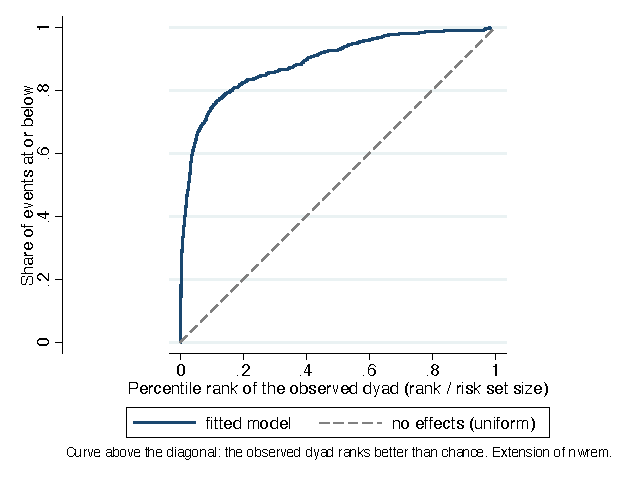
\includegraphics[width=.48\textwidth]{fig/es_rank.pdf}\hfill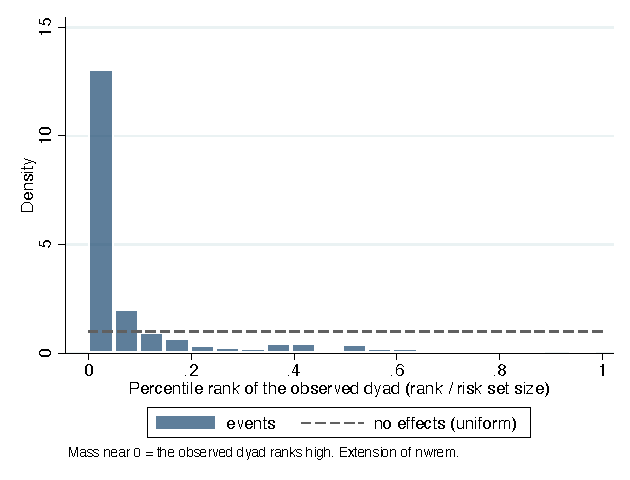
\includegraphics[width=.48\textwidth]{fig/es_rankhist.pdf}
\caption{\texttt{estat rank} (left) and \texttt{estat rank, plot(hist) bins(20)} (right) for the model of this chapter. Left: the cumulative distribution of the percentile ranks of the observed dyads; a curve above the diagonal means that the observed dyads rank better than chance. Right: their histogram against the uniform density, which is what a model without effects gives. The titles were removed with \texttt{title("")}.}\label{fig:estat-rank}
\end{figure}
The default graph is the cumulative distribution of the percentile ranks (Figure~\ref{fig:estat-rank}, left). With \opt{plot(hist)} it is the histogram of the percentile ranks, with \opt{bins()} bars (default 10), drawn against the uniform density (right). Here the mass is at the left end: for about two events in three the observed pair is within the best 5 percent of the pairs (the first bar). The results are stored in \texttt{r()}: \texttt{r(mean\_rank)}, \texttt{r(median\_rank)}, \texttt{r(mean\_pct\_rank)}, \texttt{r(hit)}, \texttt{r(hit\_model)}, \texttt{r(hit\_null)}, \texttt{r(mean\_logp)}, \texttt{r(mean\_logp\_null)}, \texttt{r(mean\_risksize)}, \texttt{r(N)} and \texttt{r(topk)}.

\section{Activity of the actors: \texttt{estat actors}}\label{sec:estat-actors}

\texttt{estat actors} compares, for every actor, the number of events observed as sender and as receiver with the number that the model expects: the sum over the events of the model probability that the actor is the sender (receiver) of the event; under the waiting-time likelihood, the summed rate integrals.
\showlog{es_actors}
The table reports, for each role, the correlation of the observed and the expected counts and the sum of the squared Pearson residuals, $(\text{observed}-\text{expected})/\sqrt{\text{expected}}$. The sums describe the fit; they are not a test, because the events are not independent draws given the effects. Here the receivers are reproduced well (correlation 0.86) and the senders poorly (0.41): with these effects the model reproduces who is written to much better than who writes. The counts of all actors are in the matrix \texttt{r(actors)}, one row per actor in the order of the network, with the columns \texttt{obs\_sender}, \texttt{exp\_sender}, \texttt{obs\_receiver} and \texttt{exp\_receiver}; \opt{list} lists them. The first rows:
\showlog{es_actors_list}
\begin{figure}[t]
\centering
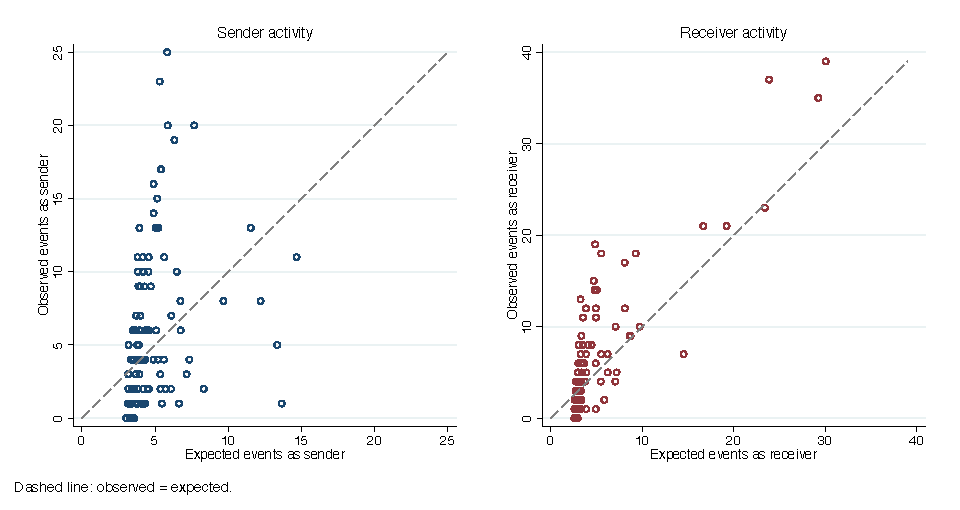
\includegraphics[width=\textwidth]{fig/es_actors2.pdf}
\caption{\texttt{estat actors} for the model of this chapter: expected (horizontal) and observed (vertical) number of events per actor, as sender (left) and as receiver (right). The dashed line is the 45 degree line, on which observed and expected counts agree. Both axes of a panel start at 0 and have the same range, and the panels are square.}\label{fig:estat-actors}
\end{figure}
After a fit with \opt{interval} the expected counts are summed rate integrals of a model without a baseline rate, so their total need not equal the observed number of events, and a level far off says that the effects cannot reproduce the overall event rate; the table says so in a note under it. Judge such a fit by the correlations, not by the levels. For the waiting-time fit of Section~\ref{sec:estat-time}:
\showlog{es_actint}
The graph is a scatter plot with the 45 degree line (Figure~\ref{fig:estat-actors}). By default there are two panels, one for the senders and one for the receivers; \opt{role(sender)} or \opt{role(receiver)} draws one panel only in the graph (the table and \texttt{r()} always hold both roles), and \opt{labels} labels the points with the names of the actors. Both axes of a panel run from 0 to the same maximum and the panel is square, so that the 45 degree line is the diagonal; \opt{noequal} lets the axes have different ranges. The footnote of the graph is one short line, so that the graph fits a width of 3.6 inches. The results in \texttt{r()} are \texttt{r(n\_actors)}, \texttt{r(corr\_sender)}, \texttt{r(corr\_receiver)}, \texttt{r(chi2\_sender)}, \texttt{r(chi2\_receiver)} and the matrix \texttt{r(actors)}.

\section{The course over time: \texttt{estat time}}\label{sec:estat-time}

\texttt{estat time} compares observed and expected quantities over the sequence of events, in \opt{bins()} bins of equally many consecutive events (deciles by default; at most the number of events). What is compared depends on the likelihood.

\paragraph{Ordinal likelihood.} The ordinal likelihood has no time scale. For each bin the table shows the number of events whose observed dyad is among the $k$ most likely dyads of the risk set (\opt{topk()}, default 10; ties are split) and the number expected under the model.
\showlog{es_time}
The bins are of 78 or 79 events. The observed number of top-10 hits is small and falls over the period (4, 4, 4, 3, 4, 0, 2, 1), the expected one is about ten per bin after the first, where it is 18.8. The model finds the observed pair among its best ten less often than it expects, in every bin and increasingly so toward the end. The bin boundaries and the counts are in the matrix \texttt{r(bins)}, one row per bin, with the columns \texttt{events}, \texttt{time\_from}, \texttt{time\_to}, \texttt{observed} and \texttt{expected}; \texttt{r(n\_bins)}, \texttt{r(topk)}, \texttt{r(obs\_total)} and \texttt{r(exp\_total)} hold the number of bins, $k$ and the totals.
\showlog{es_timeret}

\paragraph{Waiting-time likelihood.} With \opt{interval} the bins show the number of events and the integrated rate of the model over the intervals that end with those events; the last bin also carries the final interval up to \opt{endtime()}. The model has no baseline rate, so a level of the expected curve that is far from the observed one says that the effects cannot reproduce the overall rate of events. The example uses the fit of Section~\ref{sec:ex-interval} (the ties of the times removed, the time in units in which the null model has the rate one):
\begin{lstlisting}
. nwrem mail2, nodsnd nidrec frpsndsnd interval starttime(0) endtime(0.0305)
. estat time, bins(8) noplot
\end{lstlisting}
\showlog{es_interval}
With 628 events observed and 776 expected, the level is about right overall, but the expected counts differ strongly from bin to bin: the fifth bin, which contains a long interval without e-mails (about 0.8 days, from day 3.57 to day 4.34 in the ordinal table above), carries 331 expected events against 78 observed, because the effects have no way to make the rate drop in a quiet period.
\begin{figure}[t]
\centering
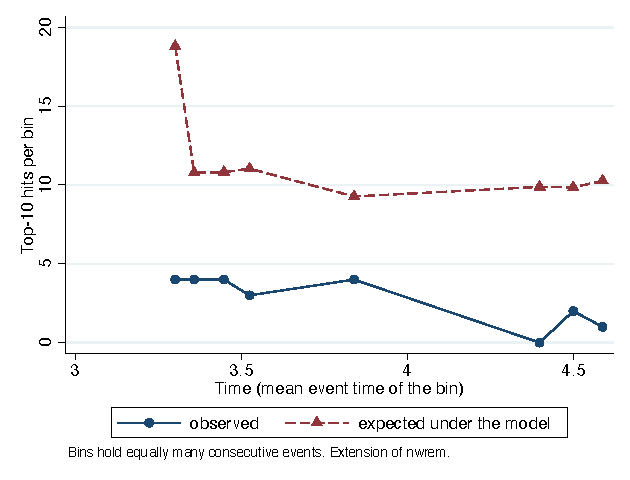
\includegraphics[width=.48\textwidth]{fig/es_time.pdf}\hfill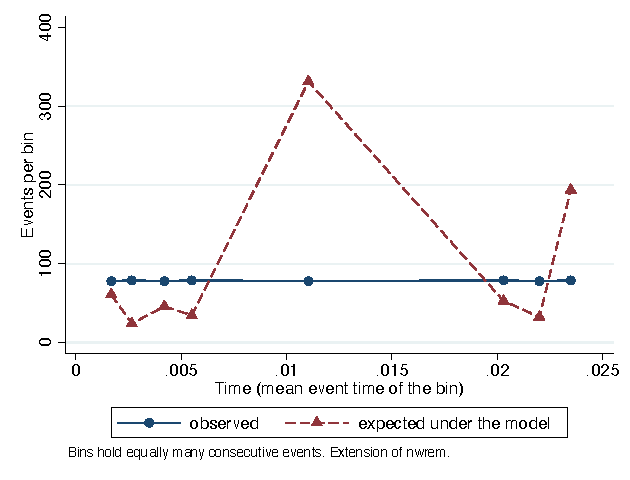
\includegraphics[width=.48\textwidth]{fig/es_timeint.pdf}
\caption{\texttt{estat time, bins(8)}. Left: after the ordinal fit, the number of top-10 hits per bin, observed and expected under the model (horizontal axis: mean event time of the bin, in days). Right: after the waiting-time fit, the number of events per bin, observed and expected (the time is in the unit of the fit).}\label{fig:estat-time}
\end{figure}
The graph (Figure~\ref{fig:estat-time}) plots the observed and the expected quantity against the mean event time of the bin, with the bins in order.
